\section{Linear Manifold Clustering}
\label{sc:lmclus}

The cluster ideal in Linear Manifold Clustering is a linear manifold.
A linear manifold of dimension zero is a point. A linear manifold of dimension 1
is a line. A linear manifold of dimension 2 is a plane. In general,
a linear manifold is a translated subspace.
The dimension of the linear manifold is the dimension of the subspace.
K-means is a special case of linear manifold clustering where
the linear manifold has dimension zero.

Linear manifold clustering is appropriate in the case that there are
linear dependencies among the variables, each cluster having a different number
and different kinds of linear dependencies.
Let us take an example to make this clear.  Suppose that we are in a three
dimensional space with three clusters. The first two clusters have one linear
dependency. Their  linear manifolds  are planes.
In our example the planes are parallel. The third cluster has
two linear dependencies. Its linear manifold is a line. The observed data points
can be thought of as points whose ideals are on their manifolds, but were
slightly perturbed off their manifolds, see Fig.~\ref{fig:lm-demo}.

\begin{figure}[h]
\IfClass{IEEEtran}{\vspace*{-12pt}}{}
\centering
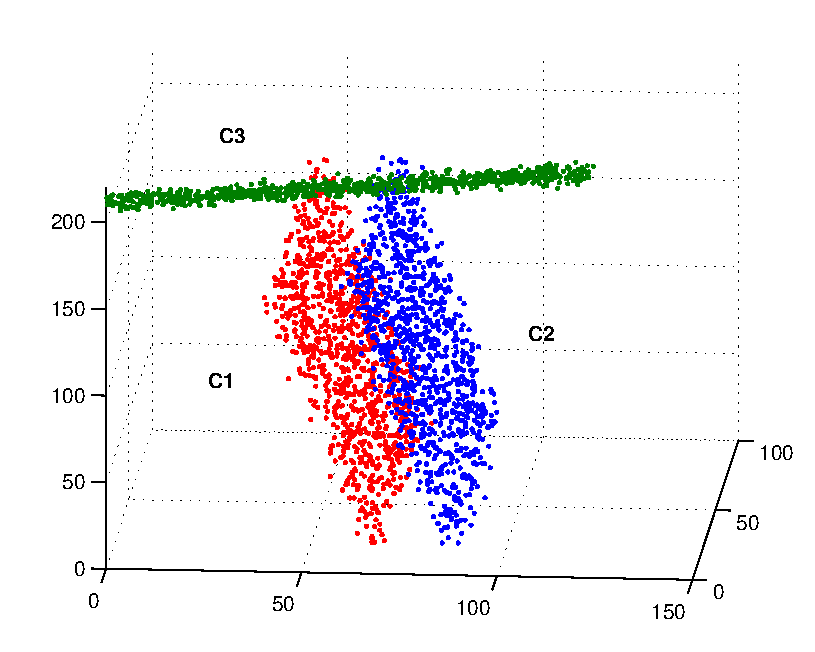
\includegraphics[width=3.5in]{img/LmDemo}
\IfClass{IEEEtran}{\vspace*{-25pt}}{}
\caption{Example of points forming three linear manifold clusters.
The green cluster is one dimensional. The blue and red clusters are
two dimensional and parallel \cite{Haralick:2007rt}.}
\label{fig:lm-demo}
\end{figure}

Linear manifold clusters \cite{Haralick:2007rt} can be found by a stochastic
search procedure, beginning with the one dimensional linear manifold clusters
and proceeding to higher dimensional clusters. A one dimensional linear manifold
is determined by two points. The stochastic search samples two points from
the data set, forms the manifold, and then the distances from all points to the
discovered manifold are calculated. If the manifold is indeed one that has many
data points close to it, the distance histogram will have a peak close to 0
distance followed by a valley and then a rise to a long fat tail or another peak
far from the origin, see Fig.~\ref{fig:dist-hist-sep}.

\begin{figure}[h]
\centering
\IfClass{IEEEtran}{
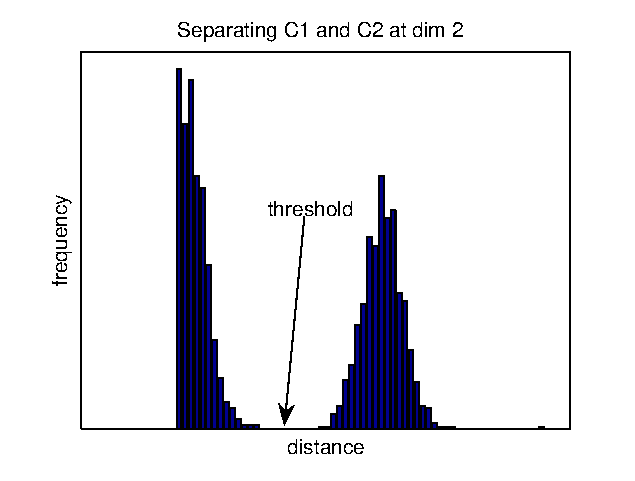
\includegraphics[width=3.5in, height=2.2in]{img/C1C2sepD2}
\vspace*{-30pt}
}{
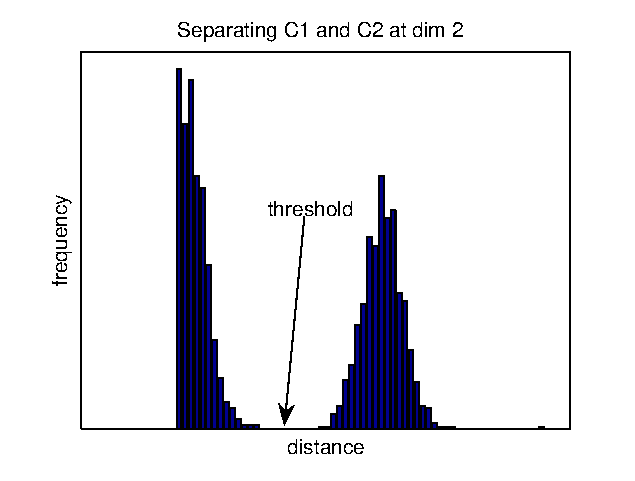
\includegraphics[width=3.5in]{img/C1C2sepD2}
}
\caption{Example of a distance to manifold histogram that shows that
a linear manifold cluster can be formed from the test manifold \cite{Haralick:2007rt}.}
\label{fig:dist-hist-sep}
\end{figure}

If this happens, then a suitable threshold can be found that separates
the data points that are near to the manifold from those data points that are
far away from the manifold. The data points that are near the manifold are
collected together and are used to make a good statistical estimate for
the manifold basis and offset. The manifold basis is given by the first
$M$ principal components of the cluster data points, where $M$  is the dimension
of the manifold. The offset can simply be the mean of the data points in
the cluster. Manifolds that do not have the right shaped distance to manifold
histograms do not get the chance to form clusters.

\IfClass{IEEEtran}{}{
Figure~\ref{fig:dist-hist-nosep} illustrates a distance to manifold histogram in
which the test manifold cannot be used to form a linear manifold cluster.
\begin{figure}[h]
\centering
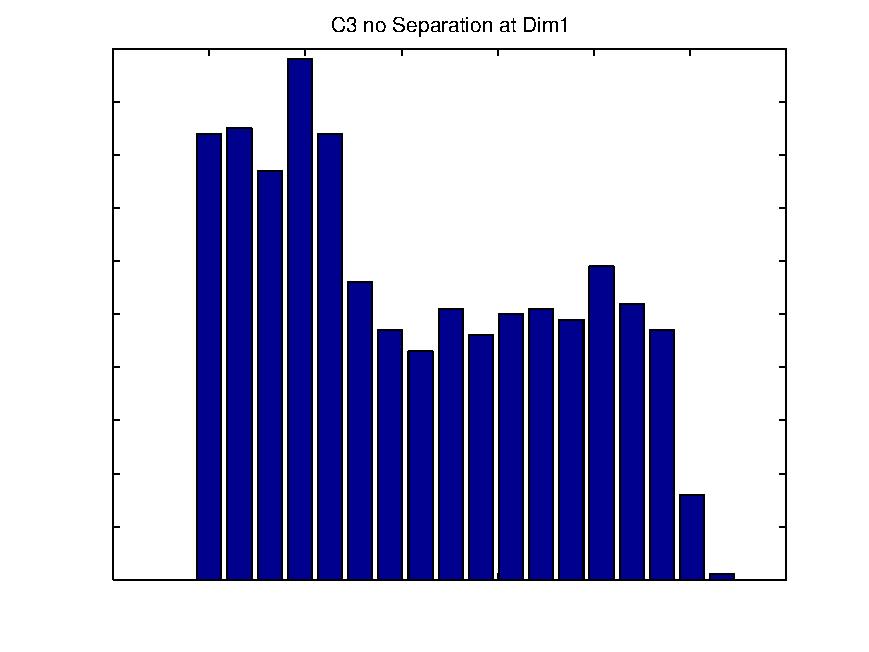
\includegraphics[width=3.5in]{img/C3nosepD1}
\caption{Illustrates a distance to manifold histogram in which the test manifold
cannot be used to form a linear manifold cluster}
\label{fig:dist-hist-nosep}
\end{figure}
}

Our linear manifold clusters must satisfy two criteria. First, the goodness of
a separation between the mode near zero and rest of the point-to-manifold
distance histogram modes should be larger then the user specified.
This criterion is fully explained in \cite{Haralick:2007rt}.
Second, the cluster compression ratio, defined as the ratio between
the linear manifold cluster description length and the uncompressed description length of the cluster, should be larger then the user defined threshold.
This criterion, in effect, acts as an internal validation the cluster
goodness-of-fit, and it is a new addition to the algorithm described
in \cite{Haralick:2007rt}.

\IfClass{IEEEtran}{}{
We extend MDL principle, so it would allow us some inexactness in
describing manifold cluster data, which can be viewed as a lossy data compression,
without loss of general understandability of the cluster structure.
%
The fundamental idea behind the MDL principle is that every regularity in
the data can be used to compress the data \cite{Grunwald:2007Gr}.
Such a description should always uniquely specify the data it describes -
hence given a description or encoding of a particular data sequence, we should
always be able to fully reconstruct data.
}
